\begin{spoken-clean}[00:00:00 - 00:00:08]
...standard, many people just use this \inlinemetanote{points at the $\subseteq$ symbol on the board}. So, I will use always this \qt{contained} without the equality sign. \inlinemetanote{The lecturer begins erasing the chalkboards to prepare for the next section}
\end{spoken-clean}

\begin{meta-note}[Topic Transition]
The lecturer erases the center and right chalkboards. He briefly writes down the exercise mentioned at the end of the previous segment before transitioning to the main topic of the second half of the lecture: Continuity.
\end{meta-note}

\begin{math-stroke}[Exercise: Completeness of Closed Subsets]
\begin{nice-box}[Exercise]
\setcounter{proposition}{49}
\begin{proposition}\label{prop:closed-subset-complete-v2}
Let $(X, d)$ be a complete metric space. If $A \subseteq X$ is a closed subset, then the metric subspace $(A, d|_A)$ is also a complete metric space.
\end{proposition}
\end{nice-box}
\end{math-stroke}

\begin{spoken-clean}[00:00:24 - 00:01:25]
Okay, let's do this because, um, maybe you will find more exciting continuous functions. Since this proof over here \inlinemetanote{points at the board} is super similar to the previous one, and is again --- you see that these proofs are one-line proofs. It's just using the definitions and manipulating around. So, I give this proof --- I left this proof as an exercise. Try to do it, again. If you understood well the definitions and you can draw a picture of what's going on, this shouldn't be too difficult. 

But it can be a bit difficult at the beginning because there are a lot of new definitions. You need to learn them. But the best is to practice with these exercises. To try to do them. Because if I do them, um, it looks like a bunch of symbols that all work sometimes, but --- but you don't interiorize the definitions. The best --- the best way is to try by yourself.
\end{spoken-clean}

\begin{spoken-clean}[00:01:25 - 00:03:41]
Okay, so I will --- I will do something more exciting now, that is continuity. Because you already know... \inlinemetanote{The lecturer erases the board and writes the heading \qt{Continuity}} Okay. Now we start to have the problems with the shadows. Maybe... so, someone, I don't remember who, complained about shadows. Now I can write here, right? Is just when the other blackboard is annoying. Okay. So, now we will see continuity.
\end{spoken-clean}

% ==========================================
% SECTION 8: CONTINUITY IN METRIC SPACES
% ==========================================
\section{Continuity in Metric Spaces}

\begin{spoken-clean}[00:03:41 - 00:05:47]
For continuity, we will define continuous maps. So, we will be in this setup. $f$ will be a map between two sets $X$ and $Y$. And they are both metric spaces. So, we will have some $X$ with its distance $d_X$, and $Y$ with its distance $d_Y$. So, many times for us, these sets will be the Euclidean space of some dimension and the Euclidean space with some other dimension, right? But it can be whatever. 

So, this is the setup. Both --- both are different metric spaces. Well, different or the same; they could be the same. Now, definition. We say that a map like this is $f$ is continuous if one of the following three equivalent properties hold true.
\end{spoken-clean}

\begin{math-stroke}[Definition: Continuity]
\setcounter{section}{2} \setcounter{subsection}{1} \setcounter{definition}{52}
\begin{definition}[Continuity]\label{def:continuity}
Let $(X, d_X)$ and $(Y, d_Y)$ be metric spaces. A mapping $f: X \to Y$ is said to be \emph{continuous} if it satisfies any of the following three equivalent conditions:
\end{definition}
\end{math-stroke}

\begin{spoken-clean}[00:05:47 - 00:07:10]
So, now I will state the three definitions of continuity, because at least with two of them you are very familiar from --- from Analysis 1, right? But I will state now postulating that they are equivalent, and later we will prove immediately that they are indeed equivalent. Right? So, the definition number one of continuity is the $\epsilon$-$\delta$ continuity that you are familiar. 

So, you know this very well for functions of one real variable. Now we need to abstract the same notion in metric spaces. So, how was the definition of --- of $\epsilon$-$\delta$? So, can someone remind me in the real line what is the definition of continuity with $\epsilon$-$\delta$? Does someone remember? \inlinemetanote{The lecturer retrieves the catch-box microphone} Yeah, good. \inlinemetanote{Tosses microphone to student}
\end{spoken-clean}

\begin{student-interaction}[Student Answer]
I think it was: a function is continuous at $x_0$ if for every $\epsilon > 0$, there exists a $\delta > 0$ such that for all $x$, if $|x - x_0| < \delta$, then $|f(x) - f(x_0)| < \epsilon$.
\end{student-interaction}

\begin{spoken-clean}[continued]
So, up to --- is very good. You said what is continuous at a point. For a continuous function is continuous at all the points, you were going to say that. But I will use directly the continuous at --- at every point. So, I will start exactly as you said. He said: well, first I will add --- since I want to be continuous at every point, I will add \qt{for every point}. For all $x$ in $X$. Okay. Next is what you said. For every $x$, given --- for all $\epsilon$ positive, exists $\delta$ positive. And now the rest of your definition used intervals and stuff that are not available in metric spaces. So, how we translate?
\end{spoken-clean}

\begin{math-stroke}[The Three Faces of Continuity]
\setcounter{proposition}{53}
\begin{proposition}[The Three Faces of Continuity]\label{prop:three-faces-continuity}
Let $f: (X, d_X) \to (Y, d_Y)$ be a map between metric spaces. The following are equivalent:
\begin{enumerate}
    \setcounter{enumi}{0} \item \emph{\texorpdfstring{$\epsilon$}{epsilon}-\texorpdfstring{$\delta$}{delta} Continuity:}
    \[ \forall x \in X, \forall \epsilon > 0, \exists \delta > 0 \text{ s.t. } \forall x' \in X, d_X(x, x') < \delta \implies d_Y(f(x), f(x')) < \epsilon \]
\end{enumerate}
\end{math-stroke}

\begin{spoken-clean}[00:08:23 - 00:10:23]
So, the notion will be that if the distance between $x$ and $x'$ is less than $\delta$, then the distance between $f(x)$ and $f(x')$ is less than $\epsilon$. And what is this distance? This distance is the distance in the space here, $X$, and this distance --- these guys belong to $Y$, so this is the distance in $Y$. Right? What else could be? Cannot be anything else. So, if you think about this, is the only way to generalize. 

Another way to say this, because this is a bit annoying to write, is a bit long, is to say that the ball --- let me put it like this: this thing, the bracket red, is the same, exactly the same as saying that the $f$ --- when I compute $f$ the image of the ball of radius $\delta$ centered at $x$ will be contained in the ball of radius $\epsilon$ centered at $f(x)$.
\end{spoken-clean}

\begin{math-stroke}[Geometric Interpretation of \texorpdfstring{$\epsilon$}{epsilon}-\texorpdfstring{$\delta$}{delta}]
The $\epsilon$-$\delta$ condition can be expressed concisely using open balls:
\begin{equation} \label{eq:continuity_balls}
f(B_\delta(x)) \subseteq B_\epsilon(f(x))
\end{equation}
\begin{explanation-of-steps}
This states that the image of a sufficiently small neighborhood around $x$ (the $\delta$-ball) must be entirely contained within a given neighborhood around the image $f(x)$ (the $\epsilon$-ball).
\end{explanation-of-steps}
\end{math-stroke}

\begin{spoken-clean}[00:10:23 - 00:12:18]
So, this is the $\epsilon$-$\delta$ definition. Second definition is with sequences. Right? Continuity with sequences. And --- and this is the same as in $\mathbb{R}$ essentially. So, if you have $x_n$ is a sequence and $x_n$ is converging to a point $x$, then the sequence of the images, that is $f(x_n)$, is convergent in the space $Y$ with limit $f(x)$. So, and a compact way to write this is that $f(x_n)$ this sequence in $n$ converges when $n$ goes to infinity to $f(x)$. And for this essentially you don't even need anything new. So, is really the same definition of $\mathbb{R}$, you plug it here and it makes sense.
\end{spoken-clean}

\begin{math-stroke}[Sequential Continuity]
\begin{enumerate}
    \setcounter{enumi}{1} \item \emph{Sequential Continuity:}
    \[ \forall (x_n)_{n \ge 0} \subset X, \quad x_n \to x \implies f(x_n) \to f(x) \]
\end{enumerate}
\end{math-stroke}

\begin{spoken-clean}[00:12:18 - 00:14:15]
And then there is the new notion of continuity, that is the topological notion of continuity, the number three, that this one is new but will be very easy to prove that is the same. And we will use this all the time, that's why I'm giving. That says that for every $V$ in $Y$ open, the pre-image $f^{-1}(V)$ that is a subset of $X$ is open. 

A map, a function is continuous is whenever you take an open set in the target and you see it back --- so you go $f^{-1}$ --- you get an open set here in the --- in the domain. Now, maybe is not obvious that the three are equivalent, but we will show that.
\end{spoken-clean}

\begin{math-stroke}[Topological Continuity]
\begin{enumerate}
    \setcounter{enumi}{2} \item \emph{Topological Continuity:}
    \[ \forall V \subseteq Y \text{ open} \implies f^{-1}(V) \subseteq X \text{ is open} \]
\end{enumerate}
\end{math-stroke}

% ==========================================
% SECTION 9: PROVING THE EQUIVALENCES
% ==========================================
\section{Proving the Equivalences}

\begin{spoken-clean}[00:14:15 - 00:16:35]
Okay, let's give the proof of this proposition. So, first I need to start to show --- so I will start with the $\epsilon$-$\delta$ continuity, right? And I will show that (1) implies (2). So, first step I will show that (1) implies (2). By assumption, I am in (1). So, my function $f$ assume that $f$ from $X$ to $Y$ is $\epsilon$-$\delta$ continuous. And let $x_n$ be a sequence converging to a point $x$. And we want to show that $f(x_n)$ converges to $f(x)$. Right? 

So, I need to use that is $\epsilon$-$\delta$ continuous. So, the first thing is to find the $\epsilon$. So, you give me the $\epsilon$ positive. What I want to prove --- let me put it like this: I want to prove that the distance between $f(x_n)$ and $f(x)$ is less than $\epsilon$ eventually for every $\epsilon$ positive. You see, I have rephrased here I have rephrased the notion of convergence. So, what I want to prove really is that $f(x_n)$ converges to $f(x)$. This is my goal.
\end{spoken-clean}

\begin{proof}[Proof of Proposition \ref{prop:three-faces-continuity}]
\begin{math-stroke}[Forward Implication \texorpdfstring{$(1) \implies (2)$}{(1) => (2)}]
\begin{ai-proof-skeleton-invisible-content}
% 1. Assume f is epsilon-delta continuous.
% 2. Let x_n -> x.
% 3. Goal: Show f(x_n) -> f(x).
% 4. For any epsilon > 0, find delta > 0 from (1).
% 5. Since x_n -> x, x_n is in B_delta(x) eventually.
% 6. By (1), f(x_n) is in B_epsilon(f(x)) eventually.
\end{ai-proof-skeleton-invisible-content}
Assume $f$ is $\epsilon$-$\delta$ continuous. Let $(x_n)_{n \ge 0}$ be a sequence in $X$ such that $x_n \to x$.
We want to show that $f(x_n) \to f(x)$, which means:
\[ \forall \epsilon > 0, \quad d_Y(f(x_n), f(x)) < \epsilon \text{ eventually} \]
Given $\epsilon > 0$, by the $\epsilon$-$\delta$ continuity of $f$:
\[ \exists \delta > 0 \text{ s.t. } f(B_\delta(x)) \subseteq B_\epsilon(f(x)) \]
Since $x_n \to x$, by the definition of convergence:
\[ x_n \in B_\delta(x) \text{ eventually} \]
Applying the function $f$ to these terms:
\[ f(x_n) \in f(B_\delta(x)) \subseteq B_\epsilon(f(x)) \text{ eventually} \]
This implies $d_Y(f(x_n), f(x)) < \epsilon$ eventually, which proves that $f(x_n) \to f(x)$.
\end{math-stroke}

\begin{spoken-clean}[00:16:35 - 00:18:12]
But I can rephrase this goal like this: I want to prove that the distance between --- sorry, last ten minutes start to... so this is with $f$. Now is correct. So, what I want to prove is that $f(x_n)$ converges to $f(x)$. This is my goal. But I am putting it in this way because here at least I see the $\epsilon$. So, given the $\epsilon$ I can find the $\delta$. So, now, given $\epsilon$ positive, by $\epsilon$-$\delta$ continuity exists some $\delta$ positive such that the ball of radius $\delta$ centered at $x$ when I apply $f$ to this ball will be contained in the ball of radius $\epsilon$ centered at $f(x)$.
\end{spoken-clean}

\begin{spoken-clean}[00:18:12 - 00:19:50]
But remember my assumption: my assumption is that $x_n$ was converging to $x$. So, since $\delta$ is positive, $x_n$ belongs to this set (i.e., $B_\delta(x)$) eventually. When I say eventually is like for $n$ very large, $x_n$ will belong to this set. But then, when I read here, the image then this implies that $f(x_n)$ belongs to the ball of radius $\epsilon$ centered at $f(x)$ eventually. So, for $n$ large. And this is what I wanted to show. Right? So, this proof shows that (1) implies (2).
\end{spoken-clean}

\begin{spoken-clean}[00:19:50 - 00:21:15]
So, since this is maybe very symbolic, let me do a picture of what is going on. So, the pictures are never rigorous but they help a lot to --- to do some intuition. And even if I don't finish the proof today of all the equivalences, is good to go step by step. So, some people work very good with these proofs that are symbols. For some people like myself, for me are very difficult to think directly with these symbols. So, when I write this kind of proof before writing to the notes or something, what I do is I do the drawing. First I do the drawing and then I translate the drawing in the symbols. Directly the symbols for some people is easy, for some people is more difficult. So, it depends on which way you reason.
\end{spoken-clean}

\begin{math-stroke}[Visualizing Continuity]
\begin{center}
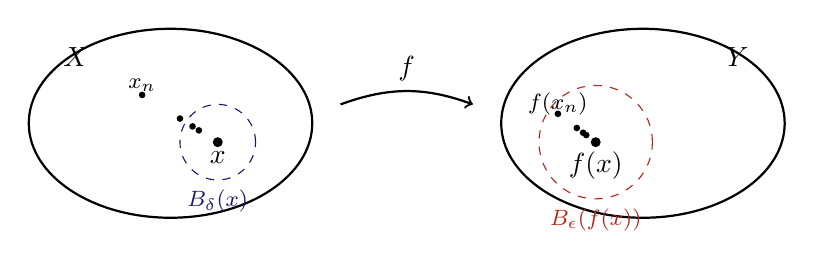
\begin{tikzpicture}[scale=1.2]
% \begin{ai-tikz-planner-invisible-content}
% 1. Background: Two metric spaces X and Y.
% 2. Midground: Point x in X and f(x) in Y.
% 3. Foreground: Sequence x_n approaching x, and f(x_n) approaching f(x).
% 4. Annotations: delta-ball in X and epsilon-ball in Y.
% \end{ai-tikz-planner-invisible-content}
    % Space X
    \draw[thick] (0,0) ellipse (1.5cm and 1cm);
    \node at (-1, 0.7) {$X$};
    \coordinate (X) at (0.5, -0.2);
    \fill (X) circle (1.5pt) node[below] {$x$};
    
    % delta-ball
    \draw[dashed, MidnightBlue] (X) circle (0.4cm);
    \node[MidnightBlue, below] at (0.5, -0.6) {\footnotesize $B_\delta(x)$};

    % Space Y
    \begin{scope}[shift={(5,0)}]
        \draw[thick] (0,0) ellipse (1.5cm and 1cm);
        \node at (1, 0.7) {$Y$};
        \coordinate (FX) at (-0.5, -0.2);
        \fill (FX) circle (1.5pt) node[below] {$f(x)$};
        
        % epsilon-ball
        \draw[dashed, BrickRed] (FX) circle (0.6cm);
        \node[BrickRed, below] at (-0.5, -0.8) {\footnotesize $B_\epsilon(f(x))$};
    \end{scope}

    % Mapping
    \draw[->, thick] (1.8, 0.2) to[bend left=20] node[midway, above] {$f$} (3.2, 0.2);

    % Sequence
    \foreach \i in {1, 2, 3, 4}
        \fill (0.5 - 0.8/\i, -0.2 + 0.5/\i) circle (1pt);
    \node at (-0.3, 0.4) {\footnotesize $x_n$};
    
    \foreach \i in {1, 2, 3, 4}
        \fill (4.5 - 0.4/\i, -0.2 + 0.3/\i) circle (1pt);
    \node at (4.1, 0.2) {\footnotesize $f(x_n)$};
\end{tikzpicture}
\end{center}
\end{math-stroke}

\begin{spoken-clean}[00:22:32 - 00:24:26]
So, what is going on in this proof? We have our first metric space $X$ and our second metric space $Y$. And we have a continuous map from $X$ to $Y$. And then what we wanted to show is that whenever we have a sequence here approaching $x$, the corresponding sequence of images will approach the $f(x)$. And we had to reason with the $\epsilon$-$\delta$. 

So, what this that this sequence converges here means literally that whenever I pick any ball --- can be very, very tiny this ball, very small --- then if I wait enough, all the elements of the sequence will fall inside of my ball. Right? If the ball is smaller, I need to wait more and more. But it always falls. And now, this is what I want to prove. So, to find this ball and to find that if I wait long enough I will be here, I need to use that the $x_n$ is convergent to $x$. So, I need to go back with this ball and see what happens with this ball, right? So, what happens is that this ball here comes from some set here around $x$ that may not be a ball. But what I know is that here there is a ball of radius $\delta$. This is the $\epsilon$-$\delta$. The blue ball. That when I compute the image of this ball, maybe it becomes a \qt{potato} or something, but is inside of my original ball. Right? And since this is a ball, the yellow points eventually will be in this ball, and then when I take the image, the points will be in my ball because the blue is inside of the bigger ball. So, with drawings is a bit clearer for some people perhaps.
\end{spoken-clean}

\begin{spoken-clean}[00:24:26 - 00:24:53]
\inlinemetanote{A student asks a question} Ah, there is some... \inlinemetanote{The lecturer retrieves the catch-box microphone}
\end{spoken-clean}

\begin{student-interaction}[Student Question]
Can I give back the cube eventually?
\end{student-interaction}

\begin{spoken-clean}[continued]
\inlinemetanote{The lecturer laughs} Ah, you need to get --- this was the question, to get back the cube? No. So, or someone else has a question. Who has a question? No, I had the cube the whole time and I was waiting for you to... ah, okay, okay.
\end{spoken-clean}

\begin{spoken-clean}[00:24:53 - 00:26:13]
Okay, now let's start to prove that (2) implies (3). To prove that (2) implies (3), we will actually prove that \qt{not 3} implies \qt{not 2}. So, again contraposition. Remember: what was 3? 3 was saying that for every $V$ subset $Y$ open, $f^{-1}(V)$ subset $X$ is open. Now, what is \qt{not 3}? The negation of this. The negation of \qt{for all} is \qt{exists}. So, \qt{not 3} means exists some $V$ subset $Y$ open such that $f^{-1}(V)$ is not open. Right?
\end{spoken-clean}

\begin{math-stroke}[Forward Implication \texorpdfstring{$(2) \implies (3)$}{(2) => (3)} (via Contraposition)]
\begin{ai-proof-skeleton-invisible-content}
% 1. Assume (3) is false.
% 2. Goal: Show (2) is false.
% 3. If (3) is false, there exists an open set V in Y such that f^{-1}(V) is not open.
% 4. Since f^{-1}(V) is not open, there exists x in f^{-1}(V) and a sequence x_n -> x such that x_n is not in f^{-1}(V) for all n.
% 5. Then f(x_n) is not in V for all n.
% 6. But f(x) is in V. Since V is open, f(x_n) cannot converge to f(x).
% 7. This contradicts (2).
\end{ai-proof-skeleton-invisible-content}
We prove $\neg (3) \implies \neg (2)$.
Assume (3) is false. Then there exists an open set $V \subseteq Y$ such that its pre-image $U = f^{-1}(V)$ is \emph{not open} in $X$.
\end{math-stroke}

\begin{spoken-clean}[00:26:13 - 00:28:12]
So, what does it mean not open? Not open, we said before. Not open, it means that exists some point $x$ in $f^{-1}(V)$ such that and there is a sequence $x_n$ convergent to $x$ --- this is what I did before, remember when I said a set is not open, there are a sequence of balls that have some point in the complement, right? So, there is a sequence $x_n$ convergent to $x$ and all the points $x_n$ do not belong or belong to the complement. Right? So, this gives me a sequence. And now, I will try to use this sequence to contradict (2).
\end{spoken-clean}

\begin{math-stroke}[Constructing the Counter-Sequence]
Since $U = f^{-1}(V)$ is not open, by Lemma \ref{lem:open-closed-sequences}:
\[ \exists x \in U \text{ and a sequence } (x_n)_{n \ge 0} \subset X \setminus U \text{ s.t. } x_n \to x \]
By the definition of the pre-image:
\begin{itemize}
    \item $x \in f^{-1}(V) \implies f(x) \in V$.
    \item $x_n \notin f^{-1}(V) \implies f(x_n) \notin V$ for all $n$.
\end{itemize}
\end{math-stroke}

\begin{spoken-clean}[00:28:12 - 00:29:34]
So, this sequence is converging to $x$, so I need to try to show that the images do not converge to $f(x)$. But then $f(x_n)$ belongs all belong to the complement of the image (i.e., actually the complement of $V$). And you notice that $V$ because $x$ belongs to $f^{-1}(V)$, $f(x)$ belongs to $V$. $f(x)$ belongs to an open set. And what I said before about open sets? That a set is open if and only if whenever you have a sequence eventually belongs to your set. But here all the sequence is in the complement of the set. So, $f(x_n)$ cannot converge to $f(x)$. Right? I use the characterization of open set by sequences. This point is inside my open set and the points are outside. So, these points can never converge to this one. Right? So, this gives that the negation of (2).
\end{spoken-clean}

\begin{math-stroke}[Contradicting Sequential Convergence]
We have $f(x) \in V$ and $f(x_n) \in Y \setminus V$ for all $n$.
Since $V$ is open, by Lemma \ref{lem:open-closed-sequences}, any sequence converging to $f(x)$ must eventually be contained in $V$.
However, our sequence $(f(x_n))$ is entirely contained in the complement $Y \setminus V$.
Therefore, $f(x_n) \not\to f(x)$.
This contradicts condition (2), completing the proof that $(2) \implies (3)$.
\end{math-stroke}
\end{proof}

\begin{spoken-clean}[00:29:34 - 00:29:59]
And since it is almost time, actually this is the easiest of the three, but the next day we will show that (3) implies (1) and we will close the --- we will close the circle. Okay? And since it is maybe the easiest, you can try to do as an exercise. If you succeed, less work for me. \inlinemetanote{The students applaud as the lecturer packs up his equipment}
\end{spoken-clean}

% [SYSTEM] Video complete.